%!TEX root = ../../main.tex


\begin{figure}[!htb]
\centering
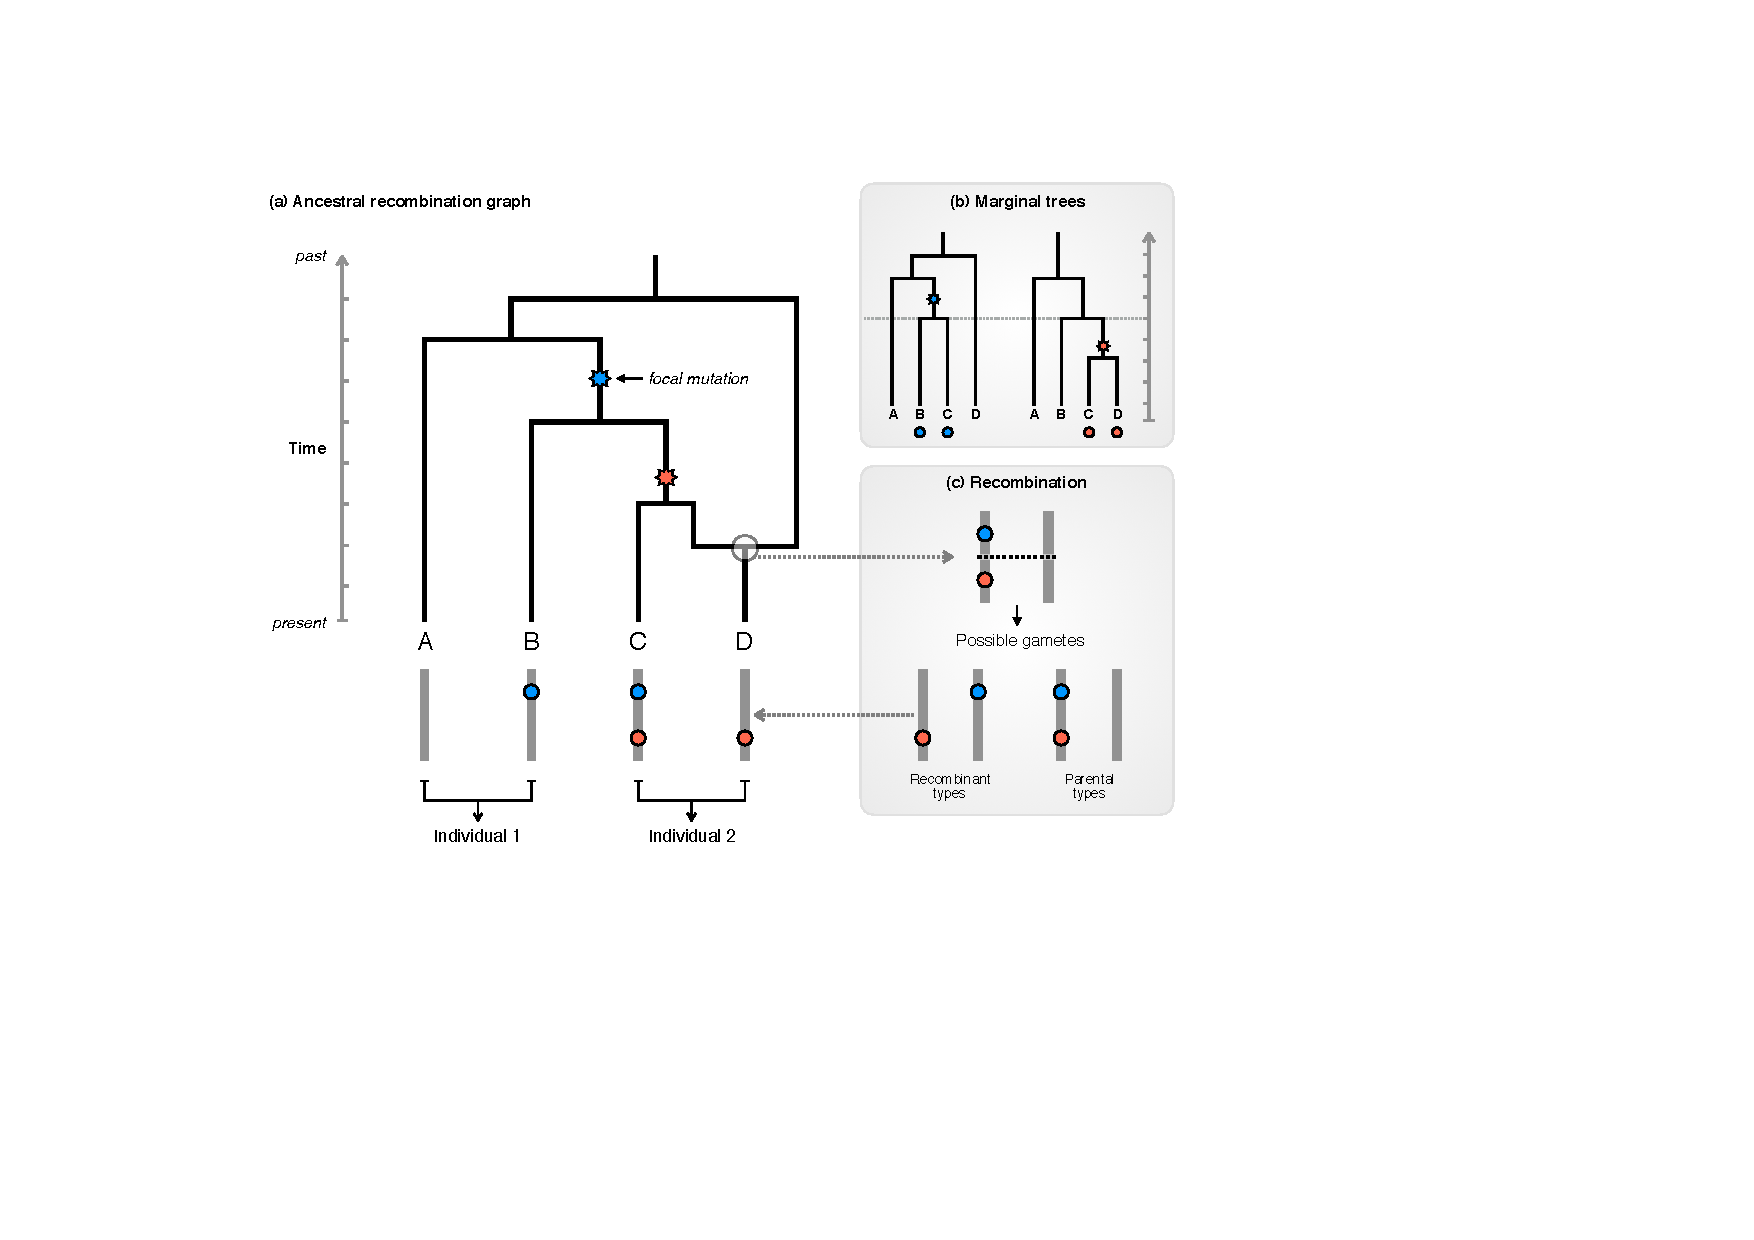
\includegraphics[width=0.9\textwidth]{./img/ch3/info_testfail_example}
\Caption{Recombination outside the focal sub-tree}
{The example shows \n{2} diploid individuals that share a focal allele (\emph{blue}) on haplotypes $B$ and $C$, which form a sub-tree within the larger genealogy.
Panel~\textbf{(a)} shows the \glsentryfull{arg} of a possible recombination history that would result in an ``unwanted'' detection of a breakpoint, due to recombination event outside the focal sub-tree.
Both the \gls{fgt} and \gls{dgt} would correctly detect a recombination event between the \n{2} sites.
However, because recombination occurred neither with haplotype $B$ nor $C$, the co-inheritance relationship between both haplotypes (relative to the focal allele) remained unbroken.
Panel~\textbf{(b)} shows the marginal trees at the \n{2} sites, corresponding to the \gls{arg} shown in Panel~(a).
Note that the \gls{tmrca} of haplotypes $B$ and $C$ in both marginal trees is identical.
Panel~\textbf{(c)} shows the possible gametes that can result from a recombination occurring between the \n{2} sites indicated.\AdditionLabel}
{fig:info_testfail_example}
\end{figure}
